% This file was created with tikzplotlib v0.10.1.
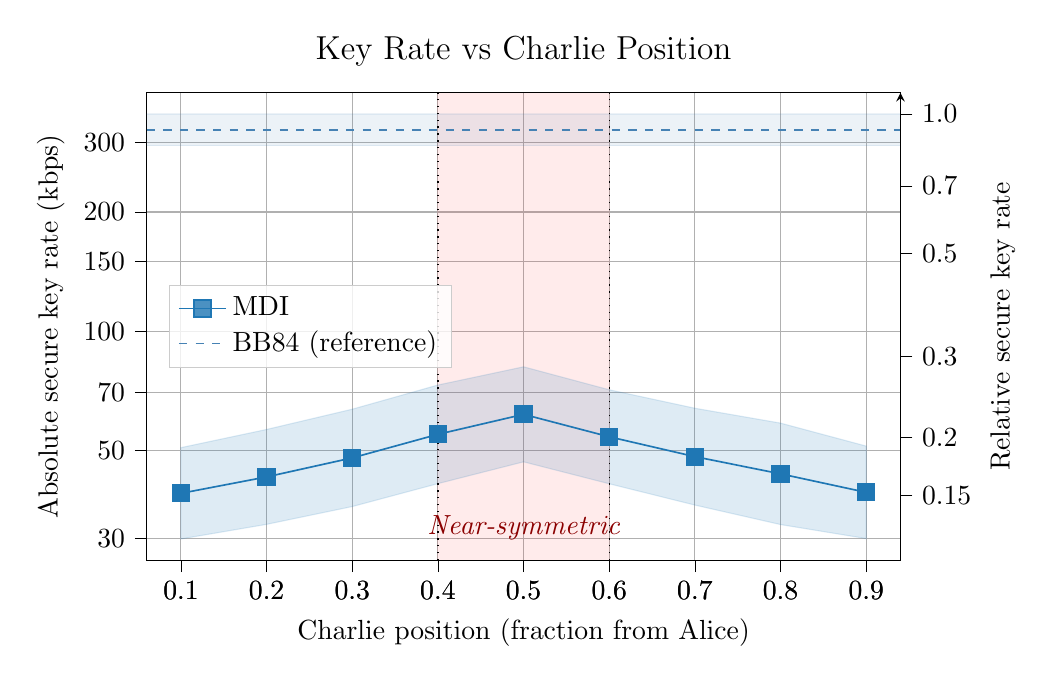
\begin{tikzpicture}
\definecolor{darkgray176}{RGB}{176,176,176}
\definecolor{darkred}{RGB}{139,0,0}
\definecolor{lightgray204}{RGB}{204,204,204}
\definecolor{steelblue}{RGB}{70,130,180}
\definecolor{steelblue31119180}{RGB}{31,119,180}
\begin{axis}[
width=0.92\linewidth,
height=0.62\linewidth,
legend cell align={left},
legend style={
  fill opacity=0.8,
  draw opacity=1,
  text opacity=1,
  at={(0.03,0.5)},
  anchor=west,
  draw=lightgray204,
  font=\fontsize{10}{12}\selectfont
},
log basis y={10},
tick align=outside,
tick pos=left,
tick label style={font=\fontsize{10}{12}\selectfont},
label style={font=\fontsize{10}{12}\selectfont},
title style={font=\fontsize{12}{14}\selectfont},
x grid style={darkgray176},
xlabel={Charlie position (fraction from Alice)},
xmajorgrids,
xmin=0.06, xmax=0.94,
xtick style={color=black},
xtick={0,0.1,0.2,0.3,0.4,0.5,0.6,0.7,0.8,0.9,1},
xticklabels={
  \(\displaystyle {0.0}\),
  \(\displaystyle {0.1}\),
  \(\displaystyle {0.2}\),
  \(\displaystyle {0.3}\),
  \(\displaystyle {0.4}\),
  \(\displaystyle {0.5}\),
  \(\displaystyle {0.6}\),
  \(\displaystyle {0.7}\),
  \(\displaystyle {0.8}\),
  \(\displaystyle {0.9}\),
  \(\displaystyle {1.0}\)
},
y grid style={darkgray176},
ylabel={Absolute secure key rate (kbps)},
ymajorgrids,
ymin=26.4049770188945, ymax=400.078803844017,
ymode=log,
ytick style={color=black},
ytick={30,50,70,100,150,200,300},
yticklabels={
  \(\displaystyle {30}\),
  \(\displaystyle {50}\),
  \(\displaystyle {70}\),
  \(\displaystyle {100}\),
  \(\displaystyle {150}\),
  \(\displaystyle {200}\),
  \(\displaystyle {300}\)
}
]
\path [draw=red, fill=red, opacity=0.08]
(axis cs:0.4,26.4049770188945)
--(axis cs:0.4,400.078803844017)
--(axis cs:0.6,400.078803844017)
--(axis cs:0.6,26.4049770188945)
--cycle;
\path [draw=steelblue31119180, fill=steelblue31119180, opacity=0.15]
(axis cs:0.1,50.8086840414235)
--(axis cs:0.1,29.877417452634)
--(axis cs:0.2,32.5255430840564)
--(axis cs:0.3,36.0743871593834)
--(axis cs:0.4,41.2136062536082)
--(axis cs:0.5,46.7797449521567)
--(axis cs:0.6,41.1761326145135)
--(axis cs:0.7,36.3851800069646)
--(axis cs:0.8,32.4853087814521)
--(axis cs:0.9,29.9455875363481)
--(axis cs:0.9,51.269720384687)
--(axis cs:0.9,51.269720384687)
--(axis cs:0.8,58.5964317946212)
--(axis cs:0.7,63.8943981387688)
--(axis cs:0.6,71.1323868499006)
--(axis cs:0.5,81.3046795054445)
--(axis cs:0.4,73.1394436918974)
--(axis cs:0.3,63.5384181905234)
--(axis cs:0.2,56.4799596545301)
--(axis cs:0.1,50.8086840414235)
--cycle;
\path [draw=steelblue, fill=steelblue, opacity=0.1]
(axis cs:0,293.973195124349)
--(axis cs:0,353.580480575196)
--(axis cs:1,353.580480575196)
--(axis cs:1,293.973195124349)
--cycle;
\addplot [semithick, steelblue31119180, mark=square*, mark size=3, mark options={solid}]
table {%
0.1 38.9619335162489
0.2 42.860720492418
0.3 47.8759803795155
0.4 54.9030075125745
0.5 61.6718101784075
0.6 54.1198354960395
0.7 48.2162750294521
0.8 43.6293843681018
0.9 39.1829286774704
};
\addlegendentry{MDI}
\addplot [semithick, steelblue, dashed]
table {%
0.06 322.402207821679
0.94 322.402207821679
};
\addlegendentry{BB84 (reference)}
\addplot [line width=0.48pt, black, dotted, forget plot]
table {%
0.4 26.4049770188945
0.4 400.078803844017
};
\addplot [line width=0.48pt, black, dotted, forget plot]
table {%
0.6 26.4049770188945
0.6 400.078803844017
};
\draw (axis cs:0.5,28) node[
  font=\fontsize{10}{12}\selectfont,
  anchor=south,
  text=darkred,
  rotate=0.0
]{\itshape Near-symmetric};
\end{axis}
\begin{axis}[
width=0.92\linewidth,
height=0.62\linewidth,
axis y line=right,
log basis y={10},
tick align=outside,
tick label style={font=\fontsize{10}{12}\selectfont},
label style={font=\fontsize{10}{12}\selectfont},
title style={font=\fontsize{12}{14}\selectfont},
title={Key Rate vs Charlie Position},
x grid style={darkgray176},
xmin=0.06, xmax=0.94,
xtick pos=left,
xtick style={color=black},
y grid style={darkgray176},
ylabel={Relative secure key rate},
ymin=0.108731309488866, ymax=1.11144474117633,
ymode=log,
ytick pos=right,
ytick style={color=black},
ytick={0.15,0.2,0.3,0.5,0.7,1},
yticklabel style={anchor=west},
yticklabels={
  \(\displaystyle {0.15}\),
  \(\displaystyle {0.2}\),
  \(\displaystyle {0.3}\),
  \(\displaystyle {0.5}\),
  \(\displaystyle {0.7}\),
  \(\displaystyle {1.0}\)
}
]
\addplot [semithick, steelblue31119180, opacity=0, mark=square*, mark size=3, mark options={solid}]
table {%
0.1 0.120848842132616
0.2 0.132941771031929
0.3 0.148497681523309
0.4 0.170293522130411
0.5 0.191288423845156
0.6 0.16786434516594
0.7 0.149553178792499
0.8 0.135325947867681
0.9 0.12153430630085
};
\addplot [semithick, steelblue31119180, opacity=0, dashed]
table {%
0.06 1
0.94 1
};
\end{axis}
\end{tikzpicture}
